\section{Components}
\label{sec:components}

A high-level overview of the architecture of the system is provided in Figure \ref{fig:architecture-diagram}. The system is made up of two components:

\begin{enumerate}
    \item \label{item:wallet}\textbf{Wallet Software}. This is a piece of software acting as a client, interacting with the chain to spend specific UTXOs depending on the required action in the collateral lifecycle. The Wallet contains the Typescript files corresponding to the ISDA CDM: these describe the properties that different objects used throughout the lifecycle must possess, such as legal documentation or different types of events. The Wallet also contains Enumerations, i.e. lists of specific named values that certain properties can take on, e.g. the type of collateral allowed in a trade can only be one described in the Eligible Collateral Enumeration. The Wallet uses the type definitions when a new contract instance is created, populating it with the desired properties agreed upon by the two counterparties (this could either be done by a Wallet held by a custodian or one of the two counterparties, the difference being that a the custodian will have already sorted disputes regarding the specifics of the contract, thus lowering if not eliminating the chances of on-chain disputes that would require additional contract updates). By storing the type definition off-chain, the system allows for easily updating the type definition should ISDA wish to do so, as opposed to a solution where the types were stored on chain and references to their addresses would have to be updated in all contract instances where they were used. It is true, on the other hand, that this poses problems regarding version mismatches: a party might update their wallet software while another might not, causing issues of interoperability. A fully on-chain solution could solve this problem by having a single source of truth for the type definitions and implementation of this alternative is suggested as future work on this dissertation.

    \item \textbf{UTXOs}. These represent the states that the collateral is in at different points in time. We define two types of UTXOs, the contract and the balance. Note that this nomenclature is just an abstraction used for explanation purposes, there are no such things as different types of UTXOs, the only differentiating factor between them being the conditions that must be satisifief for the spending to occur.
    \begin{enumerate}
        \item \textbf{Contract}. This is the 'Smart Contract' representing the collateral. It contains the business logic describing the conditions that must be satisfied to spend that collateral (e.g. that only a transaction whose signature corresponds to the private key of one of the two counterparties or the custodian can be accepted). In Bitcoin terms, this is a Pay-to-Script-Hash (P2SH), a type of ScriptPubKey, i.e. the locking script (see Section \ref{subsec:utxos} for more details), which allows for the spending of bitcoin based on the satisfaction of the script whose hash is specified within the transaction. Additionally, this is where the contract state (e.g. the amount of collateral currently represented by that UTXO denominated in a pre-specified currency, or the timestamp of the last update to the collateral state) is also stored. As every UTXO, it also contains an amount of satoshis, corresponding in this scenario to the value of the collateral. This is computed by taking into account the current USDC-to-Satoshi rate and the Mark-to-Market valuation of the collateral --- which introduces an additional exchange rate risk --- as explained in further detail on page \pageref{item:valuation}.
        
        \item \textbf{Balance}. These represent the amount of satoshis that either counterparty has available at any moment in time and from which value can be withrdrawn and transferred to the smart contract in case the valuation of the collateral drops, or conversely to which value can be transffered in the scenario where the valuation of the collateral increase and satoshis must be returned. In Bitcoin terms, these are Pay-to-Public-Key-Hash (P2PKH), a type of ScriptPubKey (see Section \ref{subsec:utxos} for more details) which locks an amount of Bitcoin to the hash of a specific public key and only a message signed with that public key can spend the Bitcoin. The hash of the public key is commonly referred to as an address.
    \end{enumerate}
\end{enumerate}


\newgeometry{top=1cm}
\begin{figure}[!h]
    \centering
    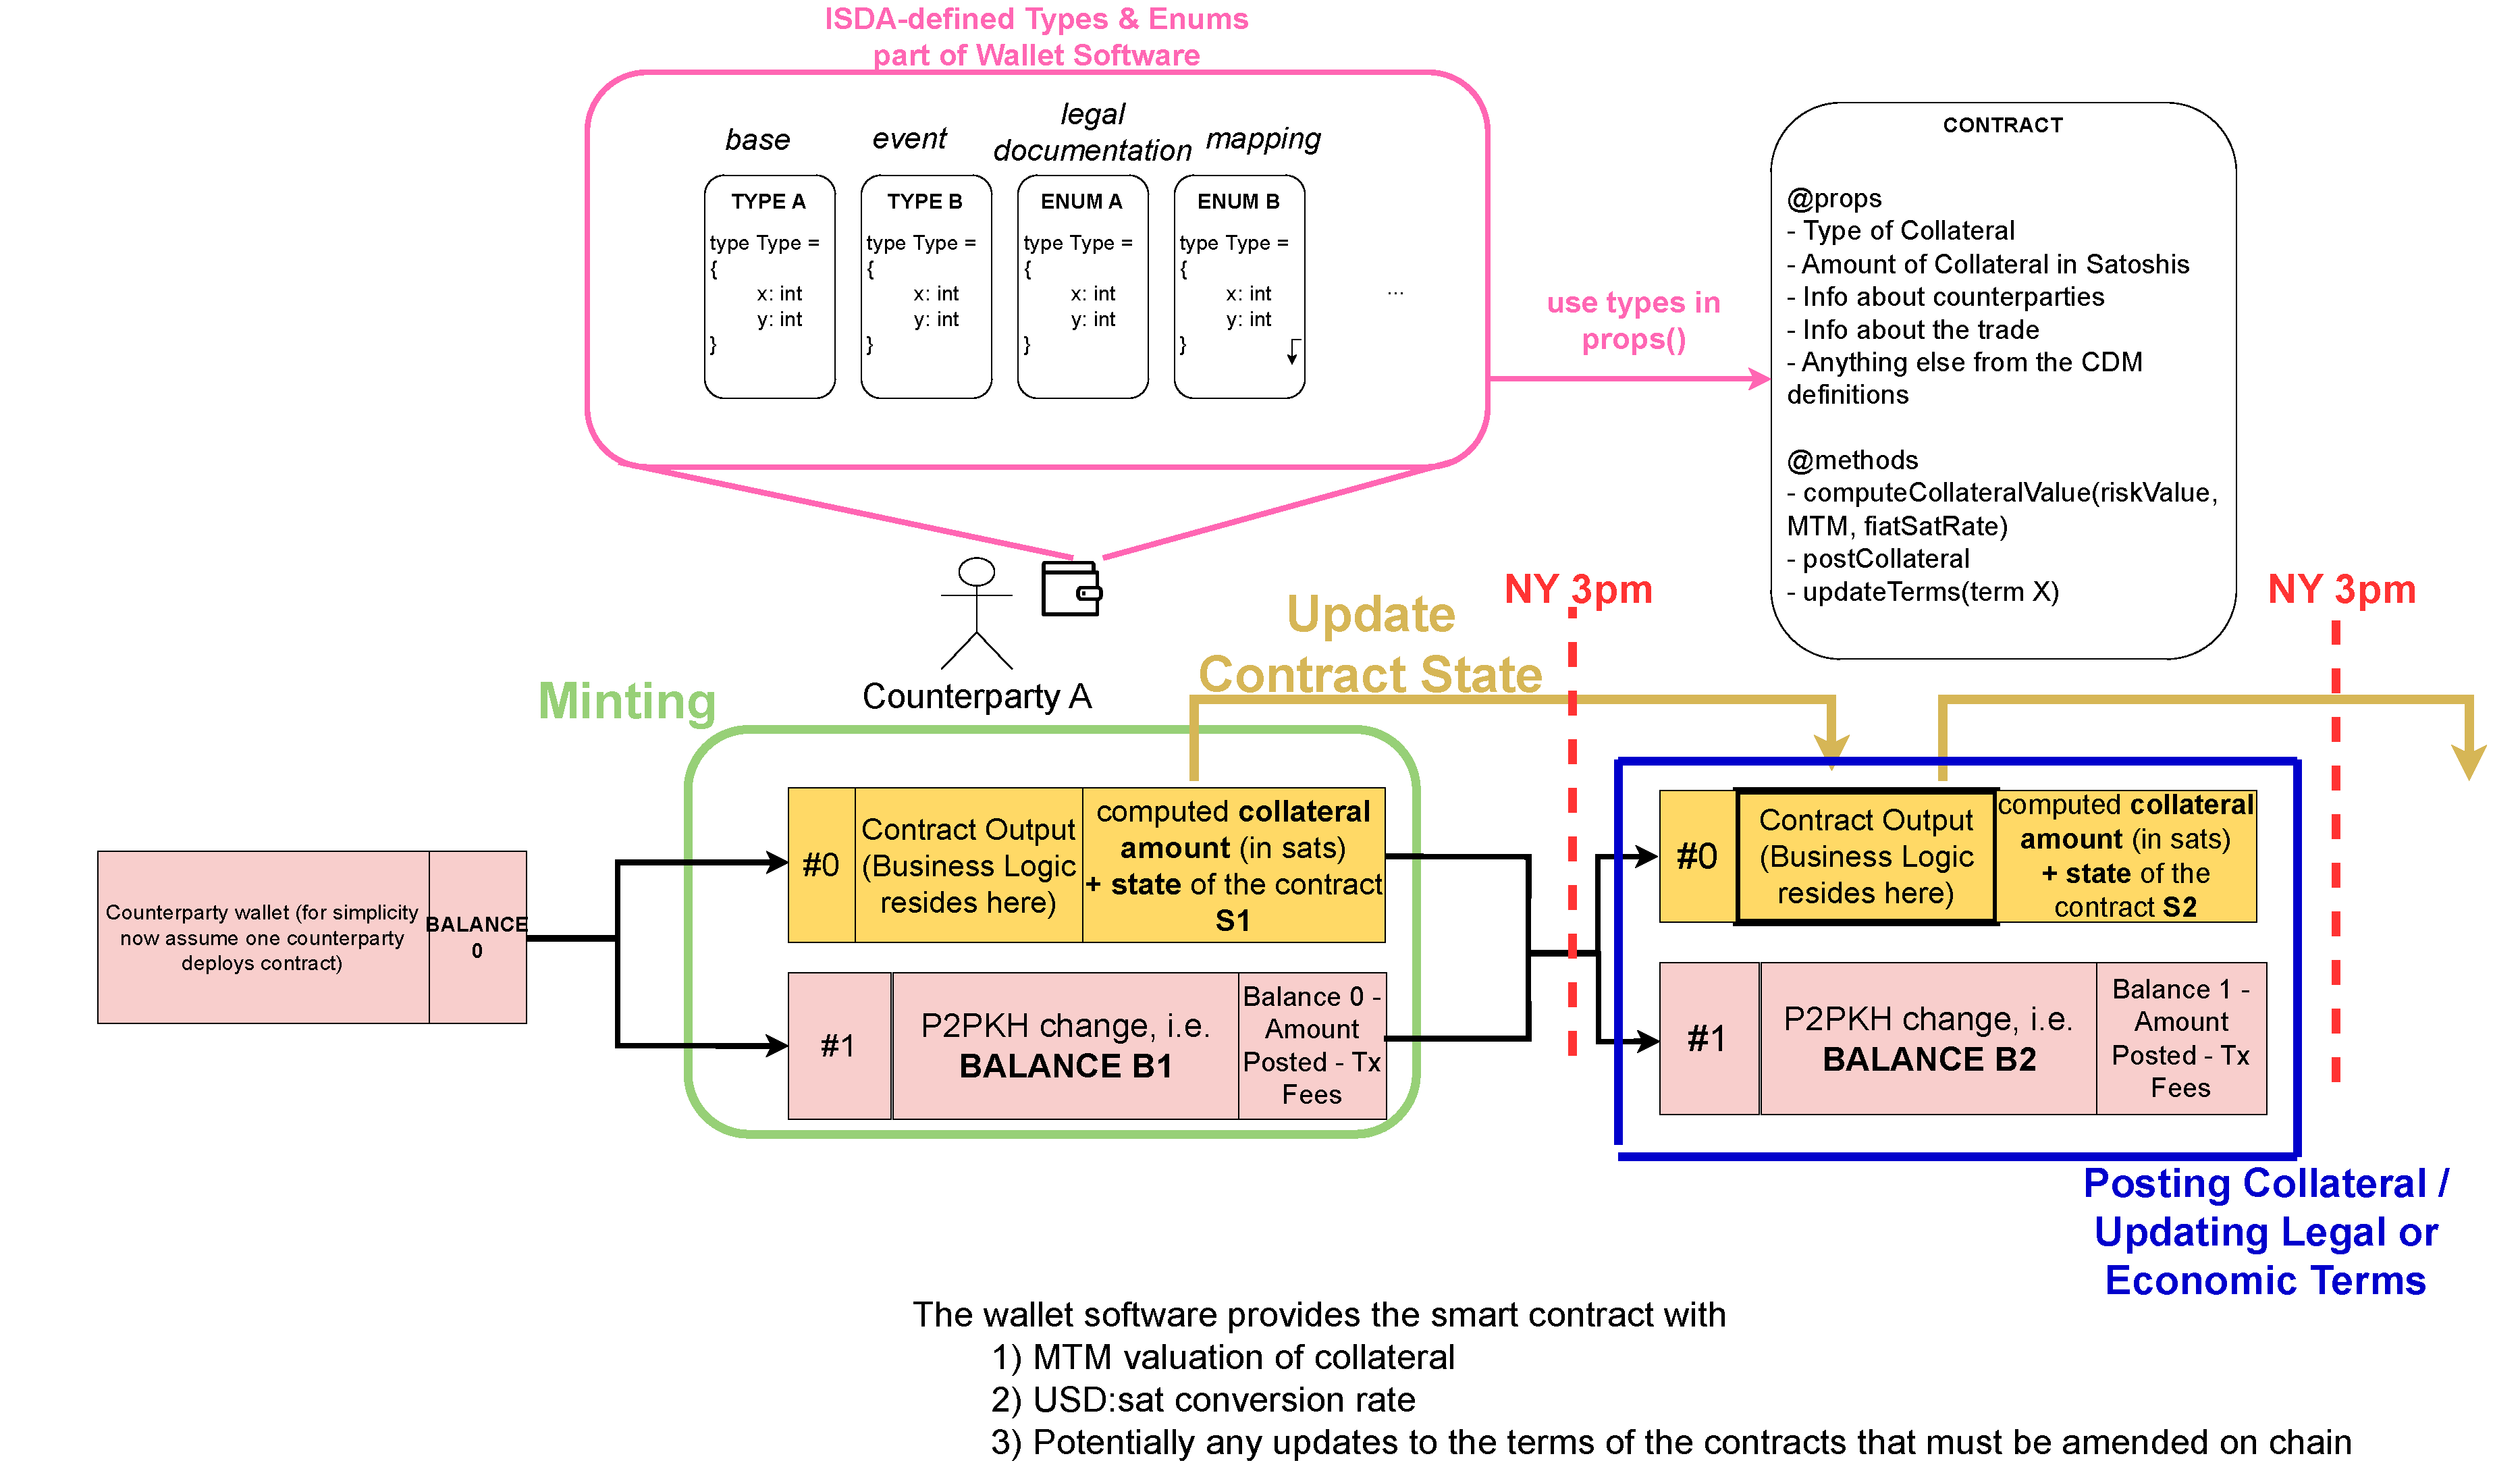
\includegraphics[angle=90, width=0.85\textwidth]{images/chapter 3/Architecture (for draft).drawio.pdf}
    \caption[High-Level Architecture Diagram]{The diagram illustrates the key components of the system. The Wallet software incorporates ISDA Common Domain Model type definitions to populate smart contracts with essential properties. UTXOs are categorized as Smart Contracts (yellow) and Balances (pink). Collateral relationships begin with Minting and can be modified through Collateral Posting or Economic Terms updates. Collateral re-evaluation occurs regularly (e.g., at 3pm New York time) to accommodate potential price fluctuations.}
    \label{fig:architecture-diagram}
\end{figure}
\restoregeometry

As the UTXOs are spent and contract state and balances are updated (details in Section \ref{sec:flow_of_events}), a chain of successive lifecycle states is formed, which together represent the entire collateral relationship between the two parties throughout time. Multiple UTXO chains, and thus series of smart contracts, can exist between the same two counterparties at the same time, each for a specific collateral relationship, and we define each one as a \textit{UTXO Set}. It is important to highlight that the system has checks in place to verify that a piece of collateral pledged in one UTXO Set cannot be utilised in another UTXO Set. By inspecting a UTXO Set, the entire history of the relationship can be inspected and thus audited, easing the job of regulatory compliance. Figure \ref{fig:custodian} shows a visual representation of UTXO Sets where a custodian still plays the role of a middleman between the two counterparties and holds assets on their behalf, thus being responsible for interacting with the chain and creating the UTXO Sets. The relevance of the figure of the custodian in this context is dicussed in further detail in Section \ref{fig:custodian}.

\begin{figure}[!h]
    \centering
    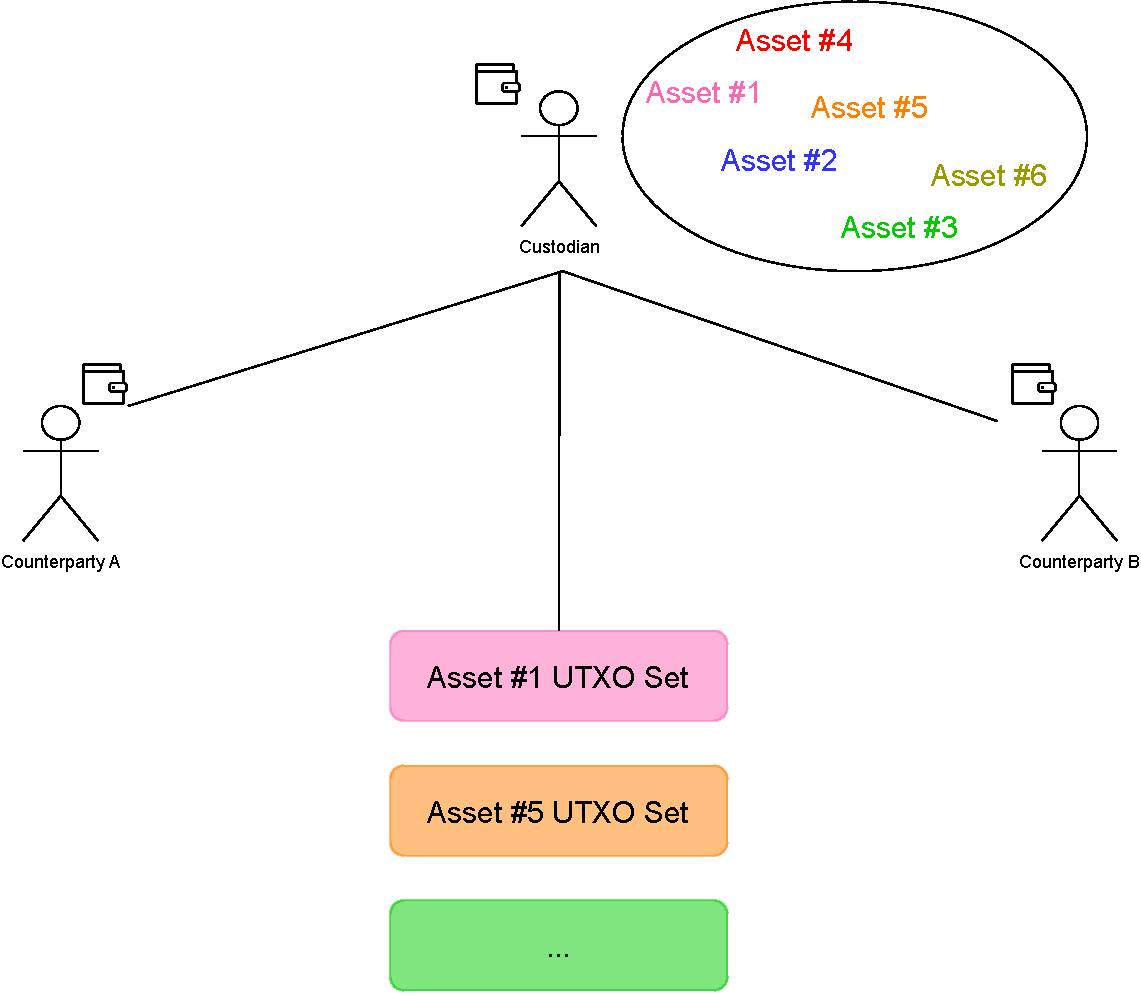
\includegraphics[width=0.5\textwidth]{images/chapter 3/custodian.drawio.pdf}
    \caption[UTXO Sets]{The Custodian wallet manages tokenised assets for counterparties. UTXOs linked to the same collateral are organized in UTXO Sets. An unlimited number of distinct UTXO Sets can exist between the same two counterparties. The diverse colors within the image represent the various assets held by the custodian, all of which can be pledged as part of a single UTXO Set at any given moment. Upon termination of a collateral relationship, the pledged assets become available for use in another UTXO Set.}
    \label{fig:custodian}
\end{figure}



